\section{Versuchsaufbau}

\begin{figure}[H]
\begin{center}
  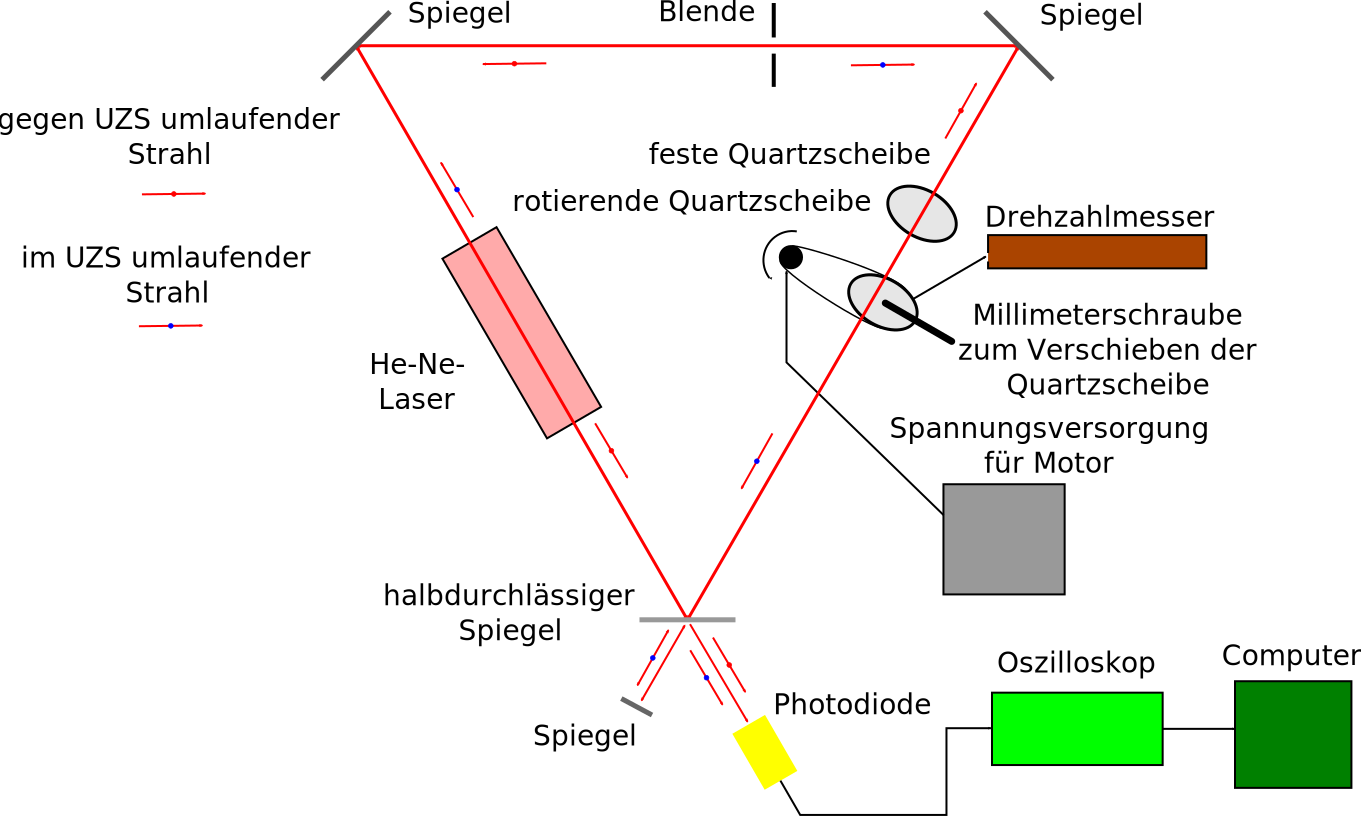
\includegraphics[width=\textwidth]{../img/aufbau.pdf}
  \caption{Aufbau zur Messung des Hanle-Effekts.}
  \label{img:aufbau}
\end{center}
\end{figure}

\autoref{img:aufbau} zeigt den Aufbau, der für die Messungen verwendet wird.
Das Licht einer Quecksilberdampflampe wird kollimiert,
fällt auf einen Interferenzfilter (Durchlassbereich 250\,nm bis 260\,nm, für die 253.7\,nm-Linie)
und wird linear polarisiert. Die Polarisationsrichtung ist einstellbar.
Eine weitere Linse fokussiert den Strahl,
der dann in einen Metallkasten fällt.
Dort befindet sich eine mit Quecksilber gefüllte Resonanzzelle,
die die Strahlung absorbiert.
Die Strahlung, die im 90$^\circ$-Winkel zur Strahlrichtung emittiert wird,
fällt in ein Alurohr und gelangt so in einen Photomultiplier,
dessen Ausgangssignal verstärkt und mit einem Oszilloskop angezeigt wird.\\
Die Temperatur der Resonanzzelle wird mit einem wassergekühltem Peltierelement gesteuert.
Zur Vermeidung von Störfeldern befindet sich dieses außerhalb der Metallbox.
Mit einem freongefüllten Wärmerohr wird seine Kühlleistung an einen Kupferblock
unter der Resonanzzelle übertragen. Der Block ist über eine Wärmebrücke mit der Resonanzzelle verbunden und
auf dem Block befindet sich ein Thermoelement,
dessen Temperaturmesswert von einem Handgerät angezeigt wird.\\
Zur Erzeugung des Magnetfelds am Ort der Resonanzzelle dienen drei Helmholtz-Spulen,
deren Strom separat mit einem Netzteil eingestellt werden kann.
Das Magnetfeld der Spule, die das Magnetfeld parallel zur Strahlrichtung (x-Richtung) erzeugt,
kann mit einem Rampengenerator gesteuert werden.
Die Rampe wird ebenfalls auf dem Oszilloskop angezeigt.
Das Oszilloskop kann mit dem Computer ausgelesen werden.


